\section{Radar Measurement Characterization}
\label{sec:char}

This section characterizes the single-chip radar measurements used
for state estimation: their timing, outliers, state-dependent noise,
within-frame correlations, and residual distribution.  These properties
inform the estimator design in \autoref{sec:method}.
\autoref{tab:char} summarizes the measurements.

Radar residuals are evaluated against motion capture, independently
of the estimator's output.  The forward model in \autoref{sec:models}
predicts each return's Doppler from the reference state; this prediction
is used to unwrap aliased measurements and compute per-return residuals.

Two residual statistics are used throughout.  The first is
$\sigma_{\mathrm{rob}}$, the median absolute deviation scaled by
1.4826, which estimates the standard deviation for
Gaussian data~\cite{rousseeuw1993alternatives}; it measures the width
of the core while limiting sensitivity to outliers.  The second is the
\emph{tail mass}, the fraction of residuals with magnitude greater than
$3\sigma_{\mathrm{rob}}$, approximately 0.27\% for a zero-mean Gaussian.

\begin{table}[t]
\centering
\caption{Measured Radar Data Properties (per-return Doppler residuals
against the \ac{mocap} forward model, ground-truth de-aliased)}
\label{tab:char}
\footnotesize
\setlength{\tabcolsep}{3pt}
\begin{tabular}{@{}lccc@{}}
\toprule
Property & Slow racing & Fast racing & Backflips \\
\midrule
Returns per frame (median)          & 13    & 11    & 10 \\
Frames below 5 returns              & 6\%   & 12\%  & 9\% \\
Aliased returns                     & 2.0\% & 23.7\% & 37.8\% \\
\midrule
Raw: $\sigma_{\mathrm{rob}}$ (m/s)  & 0.097 & 0.189 & 0.354 \\
Raw: tail mass ($>3\sigma_{\mathrm{rob}}$) & 8.6\% & 17.8\% & 6.6\% \\
Non-aliased: $\sigma_{\mathrm{rob}}$ (m/s) & 0.094 & 0.138 & 0.279 \\
Aliased: $\sigma_{\mathrm{rob}}$ (m/s) & 0.62 & 0.72 & 0.52 \\
After prefilter: $\sigma_{\mathrm{rob}}$ (m/s) & 0.085 & 0.111 & 0.243 \\
After prefilter: tail mass         & 3.1\% & 5.3\% & 2.1\% \\
\midrule
Law noise floor $\sigma_0$ (m/s)    & 0.049 & 0.140 & 0.327 \\
Law bearing constant $\delta\phi_0$ & \multicolumn{3}{c}{$2.7\degree$ (shared)} \\
Frame-shared term $\sigma_c$        & 0.96  & 1.38  & 1.55 \\
\bottomrule
\multicolumn{4}{@{}p{\columnwidth}@{}}{\scriptsize Radar frame rate
$\sim$10\,Hz, \ac{imu} rate 993\,Hz on all flights.  ``After
prefilter'' = the non-aliased returns kept by the consensus prefilter
of \autoref{sec:char_outliers}; aliased returns are handled separately.
$\sigma_0$ and $\delta\phi_0$ from the per-return fit of
\autoref{sec:char_rate}, used to determine the deployed constants
(the binned fit drawn in \autoref{fig:law} gives $\delta\phi_0 = 1.7\degree$); $\sigma_c$ in units of the noise floor $\sigma_0$ (\autoref{sec:char_corr}).}
\end{tabular}
\end{table}

\subsection{Arrival Timing and Sparsity}
\label{sec:char_temporal}
The radar delivers frames at $\sim$10\,Hz without a hardware trigger.
Each frame is timestamped on arrival at the USB port; individual returns
have no separate timestamps.  Frames contain a median of 10--13 returns,
with 6--12\% containing fewer than five (\autoref{tab:char}), the minimum
used for the consensus fit.  The \ac{imu} runs asynchronously at
993\,Hz.

\emph{Consequence.}  We use a continuous-time B-spline to evaluate the
state and its derivatives at the asynchronous radar and \ac{imu}
timestamps (\autoref{sec:state}).  Sparse frames can make per-frame
ego-velocity estimates unreliable, so the estimator uses individual
Doppler returns instead of a fitted velocity measurement.

\subsection{Outliers and the Prefilter}
\label{sec:char_outliers}
Some outliers can be identified within a frame, which is usually
overdetermined (a median of 10--13 returns for a 3-DoF ego-velocity).
A return whose Doppler disagrees with the velocity the other returns
agree on can be rejected before optimization.  We use \mbox{reve's}
three-point \ac{ransac} ego-velocity consensus filter~\cite{doer2020ekf} with the default inlier threshold of
0.15\,m/s.  The returns it rejects carry a
median absolute residual several times that of the returns it keeps
(7.4$\times$ on slow racing, 5.5$\times$ on fast racing, 2.5$\times$
on backflips, where the whole frame is noisy), and it keeps 81--91\%
of the non-aliased returns (\autoref{tab:char}); deleting the same number of returns at random removes
almost no tail mass.  A sweep of the inlier band from 0.05 to
0.6\,m/s shows that tight bands retain too few returns in sparse frames,
while loose bands retain outliers, with no value clearly better than the
adopted 0.15\,m/s.

\emph{Consequence.}  The consensus prefilter rejects outliers once per
frame, before optimization.  \autoref{sec:results} evaluates its effect
by removing it.

\subsection{The Per-Return Noise Law}
\label{sec:char_rate}
The residual core width varies with speed and return geometry.  Binning
the within-frame deviations of the non-aliased returns (the law's fit
set: frames with at least five returns, $6\sigma$-clipped) by platform
speed $|\vv|$, the angle
$\theta_j$ between the ray and the velocity vector, and by the angle
$\phi_j$ of the ray off the radar boresight (\autoref{fig:law}a--c)
shows three trends on every flight: the noise
grows linearly with speed, peaks for rays perpendicular to the motion,
and increases off boresight, by $5.7$, $2.3$ and $4.3\times$ between
the innermost and outermost bins of \autoref{fig:law}c on slow racing,
fast racing and backflips.
We use the within-frame deviation
$d_j = (r_j - \bar r_f)/\sqrt{1-1/N_f}$, where $\bar r_f$ is the mean
residual of the $N_f$ retained returns in frame $f$.  Subtracting this
mean removes an additive offset shared by all returns, but not
ray-dependent reference or timing errors.  The denominator corrects
the variance reduction from mean subtraction for independent,
equal-variance per-return errors; it is approximate when variances differ.

\begin{figure}[t]
\centering
\begin{tikzpicture}[
  scale=1.5,
  font=\footnotesize,
  supp/.style={black!55, line width=0.5pt},
  scene/.style={black!40, line width=0.5pt},
  ray/.style={black!55, line width=0.5pt, densely dotted},
  rayj/.style={black, line width=0.6pt},
  wedge/.style={fill=black!12, draw=none},
  vel/.style={-{Latex[length=2.6mm]}, line width=1.4pt, geoblue},
  velpar/.style={-{Latex[length=2.0mm]}, line width=0.8pt, geoblue},
  velperp/.style={-{Latex[length=2.2mm]}, line width=1.0pt, geoorange, densely dashed},
  ang/.style={black!75, line width=0.5pt},
  lbl/.style={font=\scriptsize},
]
\definecolor{geoblue}{RGB}{31,119,180}
\definecolor{geoorange}{RGB}{217,95,2}
% side view; the radar is at S, the body is pitched 24.5 deg nose down
% (dynamic flight), the boresight a further 27.5 deg down: -52 deg
\coordinate (S) at (0,0);
% static scene: floor and a wall ahead
\draw[scene] (0.6,-2.3) -- (4.75,-2.3);
% bearing cones: they swing the ray about the radar and do not stretch it
\fill[wedge] (S) -- (-33.5:4.1) arc (-33.5:-21.5:4.1) -- cycle;
\fill[wedge] (S) -- (-67:2.45) arc (-67:-61:2.45) -- cycle;
\draw[supp] (S) -- (-33.5:4.1);  \draw[supp] (S) -- (-21.5:4.1);
\draw[supp] (S) -- (-67:2.45);   \draw[supp] (S) -- (-61:2.45);
\draw[ang, {Latex[length=1.2mm]}-{Latex[length=1.2mm]}] (-33.5:3.6) arc (-33.5:-21.5:3.6);
\draw[ang, {Latex[length=1.2mm]}-{Latex[length=1.2mm]}] (-67:2.1) arc (-67:-61:2.1);
\node[lbl, anchor=south west, inner sep=1pt] at (-21.5:3.62) {$\delta\phi_j$};
\node[lbl, anchor=east, inner sep=1pt] at (-67.5:2.15) {$\delta\phi_0$};
% the near-boresight return (static scene point on the floor)
\draw[ray] (S) -- (1.12,-2.30);  \draw[supp, fill=white] (1.12,-2.30) circle (1.1pt);
% return j: a floor point ahead, 24.5 deg above the boresight
\draw[rayj] (S) -- (4.419,-2.30); \fill (4.419,-2.30) circle (1.4pt);
\node[lbl, anchor=south west, inner sep=1pt] at (4.22,-2.17) {return $j$};
\node[lbl, rotate=-27.5, anchor=north, inner sep=1pt] at (-27.5:2.35) {$\vu_j$};
% radar boresight (sensor x), stops at the floor
\draw[supp, dashed] (S) -- (-52:2.9);
\node[lbl, rotate=-52, anchor=south east, inner sep=1pt] at (-52:2.9) {boresight};
% quadrotor icon (side view), pitched nose down, radar at the nose underside
\begin{scope}[rotate=-24.5]
\draw[black!70, line width=0.5pt, fill=white, rounded corners=1pt] (-0.70,0.04) rectangle (-0.12,0.22);
\draw[black!70, line width=0.5pt] (-0.62,0.22) -- (-0.86,0.36) (-0.20,0.22) -- (0.04,0.36);
\draw[black!70, line width=0.5pt] (-0.86,0.36) -- (-0.86,0.42) (0.04,0.36) -- (0.04,0.42);
\draw[black!70, line width=0.9pt] (-1.04,0.42) -- (-0.68,0.42) (-0.14,0.42) -- (0.22,0.42);
\end{scope}
% the radar: a thin plate at the nose whose face normal IS the boresight
\begin{scope}[rotate=-52]
\fill[black] (-0.09,-0.10) rectangle (0.0,0.10);
\end{scope}
% velocity (15 deg, length 2.4) and its decomposition on ray j
\draw[vel] (S) -- (15:2.4);
\node[lbl, geoblue, anchor=south] at (1.15,0.42) {$\vv$};
\draw[velpar] (S) -- (-27.5:1.769);
\node[lbl, geoblue, anchor=west, inner sep=0.5pt] at (1.05,-0.20) {$\vu_j^{\!\top}\vv$};
\draw[velperp] (-27.5:1.769) -- (15:2.4);
\node[lbl, geoorange, anchor=west, inner sep=1pt] at (2.05,-0.12) {$|\vv|\sin\theta_j$};
\draw[ang] ($(-27.5:1.769)+(62.5:0.08)$) -- ($(-27.5:1.769)+(62.5:0.08)+(152.5:0.08)$) -- ($(-27.5:1.769)+(152.5:0.08)$);
% the two angles on the same ray: theta against v (above), phi against the boresight (below)
\draw[ang] (-27.5:0.60) arc (-27.5:15:0.60);
\node[lbl, anchor=west, inner sep=0.5pt] at (-6:0.63) {$\theta_j$};
\draw[ang] (-52:1.25) arc (-52:-27.5:1.25);
\node[lbl, anchor=west, inner sep=0.5pt] at (-47:1.28) {$\phi_j$};
\end{tikzpicture}
\caption{Geometry behind the per-return law (Eq.~\eqref{eq:law}) in side view.
The platform moves with velocity $\vv$ past static scene points.  Return $j$ is the ray of direction $\vu_j$ from the radar to one of them.  The sensor reads only the along-ray part of the velocity, the Doppler $v_{D}=-\vu_j^{\top}\vv$ (positive for a receding target, so negative here).
A bearing error swings the ray about the radar (grey cones) and leaves its length unchanged, so to first order it projects only the transverse velocity, of magnitude $|\vv|\sin\theta_j$, into the Doppler residual.  $\theta_j$ is the angle between the ray and $\vv$.
The angular width of the cone grows off the boresight (dashed: the sensor $x$ axis, mounted $27.5\degree$ below the body's forward axis), from about $\delta\phi_0$ near the boresight to $\delta\phi_j = \delta\phi_0/\cos\phi_j$ at the off-boresight angle $\phi_j$.  This widening follows from the angle FFT's uniform binning in the direction cosine $\sin\phi$.}
\label{fig:geometry}
\end{figure}

\textbf{Derivation.}  Bearing error provides a model for these three
trends.  We derive it first in the angular form of
\autoref{fig:geometry}; the deployed weight uses the direction-cosine
form of the same law (\autoref{sec:robust}).  The sensor measures radial velocity along the \emph{true}
ray, $v_{\mathrm{meas}} = -\vu_{\mathrm{true}}^\top\vv$, while the
forward model predicts with the \emph{reported} ray,
$v_{\mathrm{pred}} = -\vu_{\mathrm{rep}}^\top\vv$.  The residual due to
the direction error $\delta\vu = \vu_{\mathrm{rep}} - \vu_{\mathrm{true}}$
is $r_j = \delta\vu^\top\vv$.  Both rays are unit vectors, so to first
order $\delta\vu$ is perpendicular to the ray, and only the transverse
velocity $\vv_\perp$, of magnitude $|\vv|\sin\theta_j$, couples into
the residual, $r_j \approx \delta\vu^\top\vv_\perp$.  For isotropic
tangent-plane error with total angular rms $\delta\phi_j$ across its
two components, the component along $\vv_\perp$ has rms
$\delta\phi_j/\sqrt2$.  The angle FFT uses uniformly
spaced bins in the \emph{direction cosine} $\sin\phi$.
Differentiating $\sin\phi$ converts
a constant direction-cosine error into the angle error
$\delta\phi_j = \delta\phi_0/\cos\phi_j$.  The bearing-error contribution is therefore
\begin{equation}
  \sigma_j = \frac{\delta\phi_0}{\sqrt2}\,
             \frac{|\vv|\sin\theta_j}{\cos\phi_j},
  \label{eq:law}
\end{equation}
which captures the speed and geometry dependence.  Each return also
contains speed-independent noise, including detection and quantization
noise.  Independent sources add in
variance, so with $q_j = |\vv|\sin\theta_j/\cos\phi_j$ the total variance
is modeled as
\begin{equation}
  \sigma_j^2 = \sigma_0^2 + (c\,q_j)^2, \qquad c = \delta\phi_0/\sqrt2,
  \label{eq:law_fit}
\end{equation}
with a noise floor $\sigma_0$ and coefficient $c$.  The deployed weight
uses the direction-cosine form in \eqref{eq:dircos}
(\autoref{sec:robust}), assigning constant error to the two resolved
cosines and fixing the third by unit norm.  The constants reported
below are fitted to that form.

\textbf{Fit and test.}  Fitted to the binned robust width of the
per-return deviations on the two racing flights (10 quantile bins per
flight, one shared coefficient and a per-flight floor), the law
reproduces the binned widths with $R^2 = 0.98$.  The
normalized deviations $d_j/\sigma_j$ provide a further check:
their robust width should be approximately 1 across bins of each input
(\autoref{fig:law}d).  The full law gives approximately flat profiles;
omitting a factor leaves a trend along the corresponding input.
The transverse factor shows
the smallest effect in \autoref{fig:law}d because most racing returns
have $\sin\theta \ge 0.5$ (73--80\%); it is retained
because it follows from the bearing-error model and improves the fit
($R^2 = 0.98$ against
$0.93$ without).  Held out of the fit, the
backflip flight keeps this width near 1 along speed and $\theta$,
but excess noise remains off boresight.
Additional terms fitted jointly to the same statistic receive zero
coefficients, including the body-rate term.  Thus body rate adds no
explanatory value to this fit after accounting for speed and geometry.

\textbf{Constants.}  Fitting the racing flights gives
$\delta\phi_0 = 2.7\degree$; adding the backflip flight with its own
floor changes this estimate by 3\%, supporting a shared coefficient.
The firmware uses 64 direction-cosine bins over the field of view;
the fitted error corresponds to approximately one bin per axis.
The noise floor varies across regimes
($\sigma_0 = 0.049/0.140/0.327$\,m/s on the three flights,
\autoref{tab:char}), collecting the speed-independent errors the law
does not model.  Possible sources include detection noise, smearing
at high body rate, and errors near the aliasing boundary.
A shared floor would confound these differences with the bearing-error
coefficient.  The solver uses the geometric mean of the two racing
floors, $\sigma_0 = 0.083$\,m/s, and
\autoref{sec:ablations} measures the sensitivity to that choice.

\emph{Consequence.}  Each return receives its own weight,
$w_j = \sigma_0^2/\sigma_j^2 = 1/(1 + (c\,q_j/\sigma_0)^2)$, from its
own geometry and the frame's speed; the weight halves at
$q_j = \sigma_0/c = 2.5$\,m/s.  Speed is obtained from the frame's
consensus ego-velocity.  The \ac{imu} is used in the radar front end
only for alias unwrapping (\autoref{sec:robust}).
The fitted model does not include a body-rate term.

\begin{figure*}[t]
  \centering
  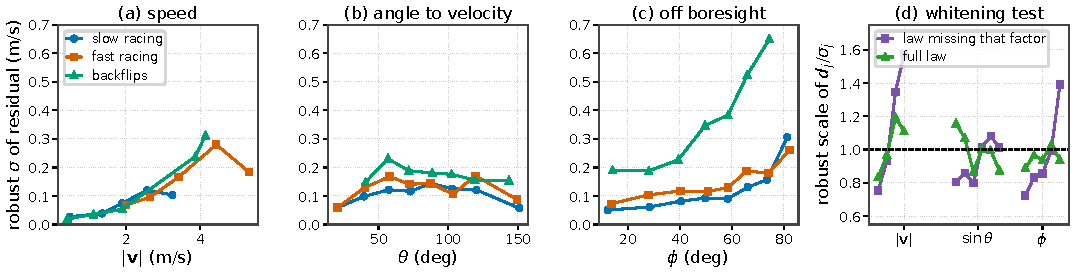
\includegraphics[width=\textwidth]{figures/law.pdf}
  \caption{The per-return noise law.  (a--c)~Robust width of the
    within-frame deviations binned by platform speed $|\vv|$, by the angle
    $\theta$ between ray and velocity, and by the angle $\phi$ off
    boresight, for the three flights: the three trends of
    \eqref{eq:law} are visible before fitting.  (d)~Model check on fast
    racing: robust scale of the normalized deviation
    $d_j/\sigma_j$ binned along each input, for the full law (green)
    and the law missing the corresponding factor (purple).  The expected
    scale is approximately 1; each missing factor leaves a trend along its
    own input.}
  \label{fig:law}
\end{figure*}

\subsection{Frame-Shared Error}
\label{sec:char_corr}
The returns of one frame share a timestamp, an attitude and an
integration interval, which can introduce correlated errors.
We estimate a frame-shared component $\sigma_c$ by separating
within-frame variation from variation in the frame means.
In units of the noise floor $\sigma_0$ of the deployed law,
$\sigma_c = 0.96/1.38/1.55$ on slow racing, fast racing
and backflips, and $0.83$--$1.02$ on the four public ICINS flights
(\autoref{sec:baselines}): the shared component is of the same order
as the per-return noise and increases across our three flight regimes.
This correlation reduces the effective number of independent
returns~\cite{kish1965survey}.

\emph{Consequence.}  Treating the returns of a frame as independent
would overstate the information in their shared component.
The estimator includes this component in the frame covariance and
whitens the residual stack as described in \autoref{sec:robust}.
We use $\sigma_c = 1.27$, the geometric mean over our three flights,
for every platform.

\subsection{Aliasing}
\label{sec:char_alias}
The firmware wraps Doppler into $\pm v_{\max} = \pm3.14$\,m/s.  Measured
against ground truth, 2.0\% of returns are aliased on slow racing,
23.7\% on fast racing and 37.8\% on backflips.
Unwrapping recovers the Doppler ambiguity but does not correct bearing
errors.  At matched speed, aliased returns have within-frame noise
2--4.6$\times$ that of non-aliased returns, with a noise floor of
$\sigma_{\mathrm{al}} \approx 0.6$\,m/s and weaker state dependence.

\emph{Consequence.}  The measurement consumed by the estimator is the
\emph{unwrapped} Doppler, selected once per frame against an
\ac{imu}-integrated velocity prediction (\autoref{sec:init}).  Selecting
the correct wrap requires the predicted radial velocity to be within
$v_{\max}$ of the true value.  Aliased returns are retained with the
reduced weight given by the measured
variance ratio $w_{\mathrm{al}} = (\sigma_0/\sigma_{\mathrm{al}})^2 = 0.019$;
\autoref{sec:results} compares this choice with full weighting and deletion.

\subsection{Doppler Residual Distribution}
\label{sec:char_noise}
A zero-mean Gaussian error model with the specified covariance yields
a covariance-weighted least-squares likelihood.  The raw residuals have
an approximately Gaussian core but heavy tails (\autoref{fig:ladder}a).
The front end treats aliased returns separately
(\autoref{sec:char_alias}) and rejects consensus outliers
(\autoref{sec:char_outliers}).  Normalizing each retained return by its
own $\sigma_j$ (\autoref{sec:char_rate}) reduces the excess mass between
$1.5\sigma$ and $3\sigma$, while the prefilter reduces the far tail
(\autoref{fig:ladder}b).

For the retained, non-aliased returns, the mass beyond $3\sigma$ is
3--10$\times$ the Gaussian value, down from
25--47$\times$ before the prefilter with one global $\sigma$.  The
remaining outlier population is not identified by the available flags:
it accounts for 1--4\% of the returns and is
5--10$\times$ wider than the core, against 6--12\% and 6--11$\times$
before.  Multipath is a possible source.  The residuals remain
approximately zero-mean and symmetric, with tails consistent with
exponential decay over the observed range.

\emph{Consequence.}  We use a Gaussian likelihood with per-return
variance $\sigma_j^2$ and frame-shared covariance
(\autoref{sec:prelim_map}, \autoref{sec:robust}).  This approximates the
core but does not model the remaining heavy tails.  A robust kernel
after prefiltering produced no measurable improvement and is not used
(\autoref{sec:ablations}).

\begin{figure*}[t]
  \centering
  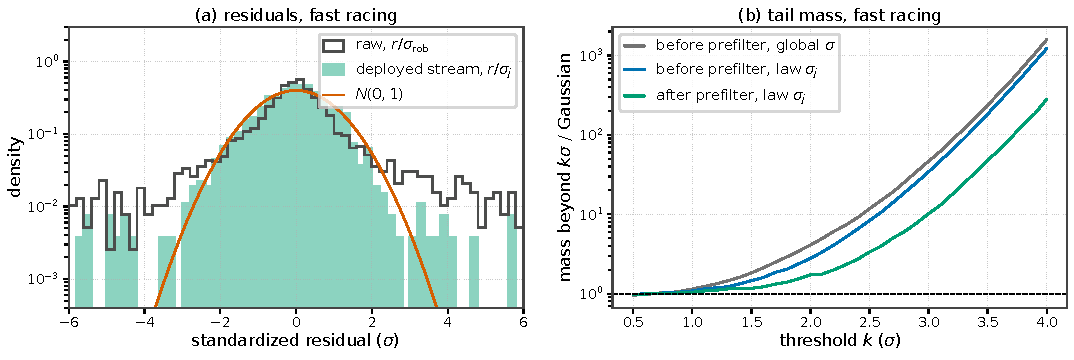
\includegraphics[width=\textwidth]{figures/ladder.pdf}
  \caption{The residual distribution before and after the front end
    (fast racing).  (a)~Standardized residuals on a log density scale:
    the raw stream in units of its $\sigma_{\mathrm{rob}}$ (grey) and
    the retained, non-aliased returns, each residual in units of its own
    $\sigma_j$ (green), against $N(0,1)$.  Aliased returns are weighted
    as their own population and are not in the green stream.
    (b)~Tail mass beyond $k\sigma$ relative to a Gaussian, for the
    non-aliased returns before the prefilter with one global $\sigma$
    (grey) and with the per-return law $\sigma_j$ (blue), and for the
    returns after the prefilter with the law (green).  Together they
    reduce the excess by an order of magnitude.  Per-return normalization
    mainly reduces the excess between $1.5\sigma$ and $3\sigma$;
    the blue and grey curves converge beyond $3.5\sigma$.
    The prefilter reduces the remaining far tail.}
  \label{fig:ladder}
\end{figure*}

\subsection{Stream Error Budgets}
\label{sec:char_budget}
The noise law sets the relative weights of radar returns.  The weights
of the radar, gyroscope, and accelerometer streams must also account
for temporal correlation.  We approximate a stream sampled at $f_s$ with integrated
autocorrelation time $\tau$ (the sum of the residual autocorrelation
over positive lags) as providing $1/\tau$ independent samples per
second.  The corresponding per-sample weight is
\begin{equation}
  \lambda^\ast = \frac{1}{\sigma^2\, f_s\, \tau},
  \label{eq:lambda_star}
\end{equation}
which for white noise ($\tau = 1/f_s$) reduces to
$1/\sigma^2$ per sample.  Both inputs are measured per stream against
the reference.  For the \ac{imu}, we use residuals within the bandwidth
represented by the splines.  Much of the raw residual energy lies above
this band: the gyroscope's in-band $\sigma$ is 0.024--0.051\,rad/s,
compared with 0.15\,rad/s before filtering.  The measured \ac{imu}
correlation times are 194--598\,ms, corresponding to approximately
2--5 independent samples per second under this approximation.
For the radar, $\sigma$ is the root-mean-square residual of the
non-aliased returns that pass the prefilter; aliased returns have their
own weight and are excluded from this estimate.  The second moment
includes the remaining outliers' contribution to the quadratic cost.
Using the robust core width instead makes the weights from the two
racing flights differ by a factor of $3.6$.

\emph{Consequence.}  Taking the geometric mean of
\eqref{eq:lambda_star} over the two racing flights gives
$\lambda_g = 3.13$, $\lambda_a = 0.0039$, and a radar weight of $2.64$
per return (\autoref{sec:robust}).  Ignoring temporal correlation would
increase the \ac{imu} weights by $f_s\tau$, a factor of several hundred,
relative to this approximation.  \autoref{sec:nees} tests the consistency
of the resulting estimator covariance.
